\documentclass{article}\usepackage[]{graphicx}\usepackage[]{xcolor}
% maxwidth is the original width if it is less than linewidth
% otherwise use linewidth (to make sure the graphics do not exceed the margin)
\makeatletter
\def\maxwidth{ %
  \ifdim\Gin@nat@width>\linewidth
    \linewidth
  \else
    \Gin@nat@width
  \fi
}
\makeatother

\definecolor{fgcolor}{rgb}{0.345, 0.345, 0.345}
\newcommand{\hlnum}[1]{\textcolor[rgb]{0.686,0.059,0.569}{#1}}%
\newcommand{\hlsng}[1]{\textcolor[rgb]{0.192,0.494,0.8}{#1}}%
\newcommand{\hlcom}[1]{\textcolor[rgb]{0.678,0.584,0.686}{\textit{#1}}}%
\newcommand{\hlopt}[1]{\textcolor[rgb]{0,0,0}{#1}}%
\newcommand{\hldef}[1]{\textcolor[rgb]{0.345,0.345,0.345}{#1}}%
\newcommand{\hlkwa}[1]{\textcolor[rgb]{0.161,0.373,0.58}{\textbf{#1}}}%
\newcommand{\hlkwb}[1]{\textcolor[rgb]{0.69,0.353,0.396}{#1}}%
\newcommand{\hlkwc}[1]{\textcolor[rgb]{0.333,0.667,0.333}{#1}}%
\newcommand{\hlkwd}[1]{\textcolor[rgb]{0.737,0.353,0.396}{\textbf{#1}}}%
\let\hlipl\hlkwb

\usepackage{framed}
\makeatletter
\newenvironment{kframe}{%
 \def\at@end@of@kframe{}%
 \ifinner\ifhmode%
  \def\at@end@of@kframe{\end{minipage}}%
  \begin{minipage}{\columnwidth}%
 \fi\fi%
 \def\FrameCommand##1{\hskip\@totalleftmargin \hskip-\fboxsep
 \colorbox{shadecolor}{##1}\hskip-\fboxsep
     % There is no \\@totalrightmargin, so:
     \hskip-\linewidth \hskip-\@totalleftmargin \hskip\columnwidth}%
 \MakeFramed {\advance\hsize-\width
   \@totalleftmargin\z@ \linewidth\hsize
   \@setminipage}}%
 {\par\unskip\endMakeFramed%
 \at@end@of@kframe}
\makeatother

\definecolor{shadecolor}{rgb}{.97, .97, .97}
\definecolor{messagecolor}{rgb}{0, 0, 0}
\definecolor{warningcolor}{rgb}{1, 0, 1}
\definecolor{errorcolor}{rgb}{1, 0, 0}
\newenvironment{knitrout}{}{} % an empty environment to be redefined in TeX

\usepackage{alltt}
\usepackage{amsmath} %This allows me to use the align functionality.
                     %If you find yourself trying to replicate
                     %something you found online, ensure you're
                     %loading the necessary packages!
\usepackage{amsfonts}%Math font
\usepackage{graphicx}%For including graphics
\usepackage{hyperref}%For Hyperlinks
\usepackage[shortlabels]{enumitem}% For enumerated lists with labels specified
                                  % We had to run tlmgr_install("enumitem") in R
\hypersetup{colorlinks = true,citecolor=black} %set citations to have black (not green) color
\usepackage{natbib}        %For the bibliography
\setlength{\bibsep}{0pt plus 0.3ex}
\bibliographystyle{apalike}%For the bibliography
\usepackage[margin=0.50in]{geometry}
\usepackage{float}
\usepackage{multicol}

%fix for figures
\usepackage{caption}
\newenvironment{Figure}
  {\par\medskip\noindent\minipage{\linewidth}}
  {\endminipage\par\medskip}
\IfFileExists{upquote.sty}{\usepackage{upquote}}{}
\begin{document}

\vspace{-1in}
\title{Lab 05 -- MATH 240 -- Computational Statistics}

\author{
  Reagan Sernick \\
  Affiliation  \\
  Department  \\
  {\tt rsernick@colgate.edu}
}

\date{2/27/25}

\maketitle

\begin{multicols}{2}
\begin{abstract}
In this lab, we took the data we extracted from last lab and interpreted it in terms of wether the data for \emph{Allentown} was within range, outlying, or out of range of the data from each of the artists that contributed. In the end this will give us an idea of which artist contributed the most.
\end{abstract}

\noindent \textbf{Keywords:} 

\section{Introduction}

The purpose of this lab, and the two leading up to it, was to determine which artist contributed the most on \emph{Allentown} of the contributing artists. To do this, we had to take the data from the previous lab and interpret it in a meaningful way.

\section{Methods}

The data we used from this lab came from Essentia, Essentia Models, and LIWC. These programs help model data from a song's waveform and lyrics in a quantitative way.

\subsection{}



\pagebreak

\onecolumn

\section{Results}







\begin{figure}[H]
\begin{center}
\begin{knitrout}
\definecolor{shadecolor}{rgb}{0.969, 0.969, 0.969}\color{fgcolor}
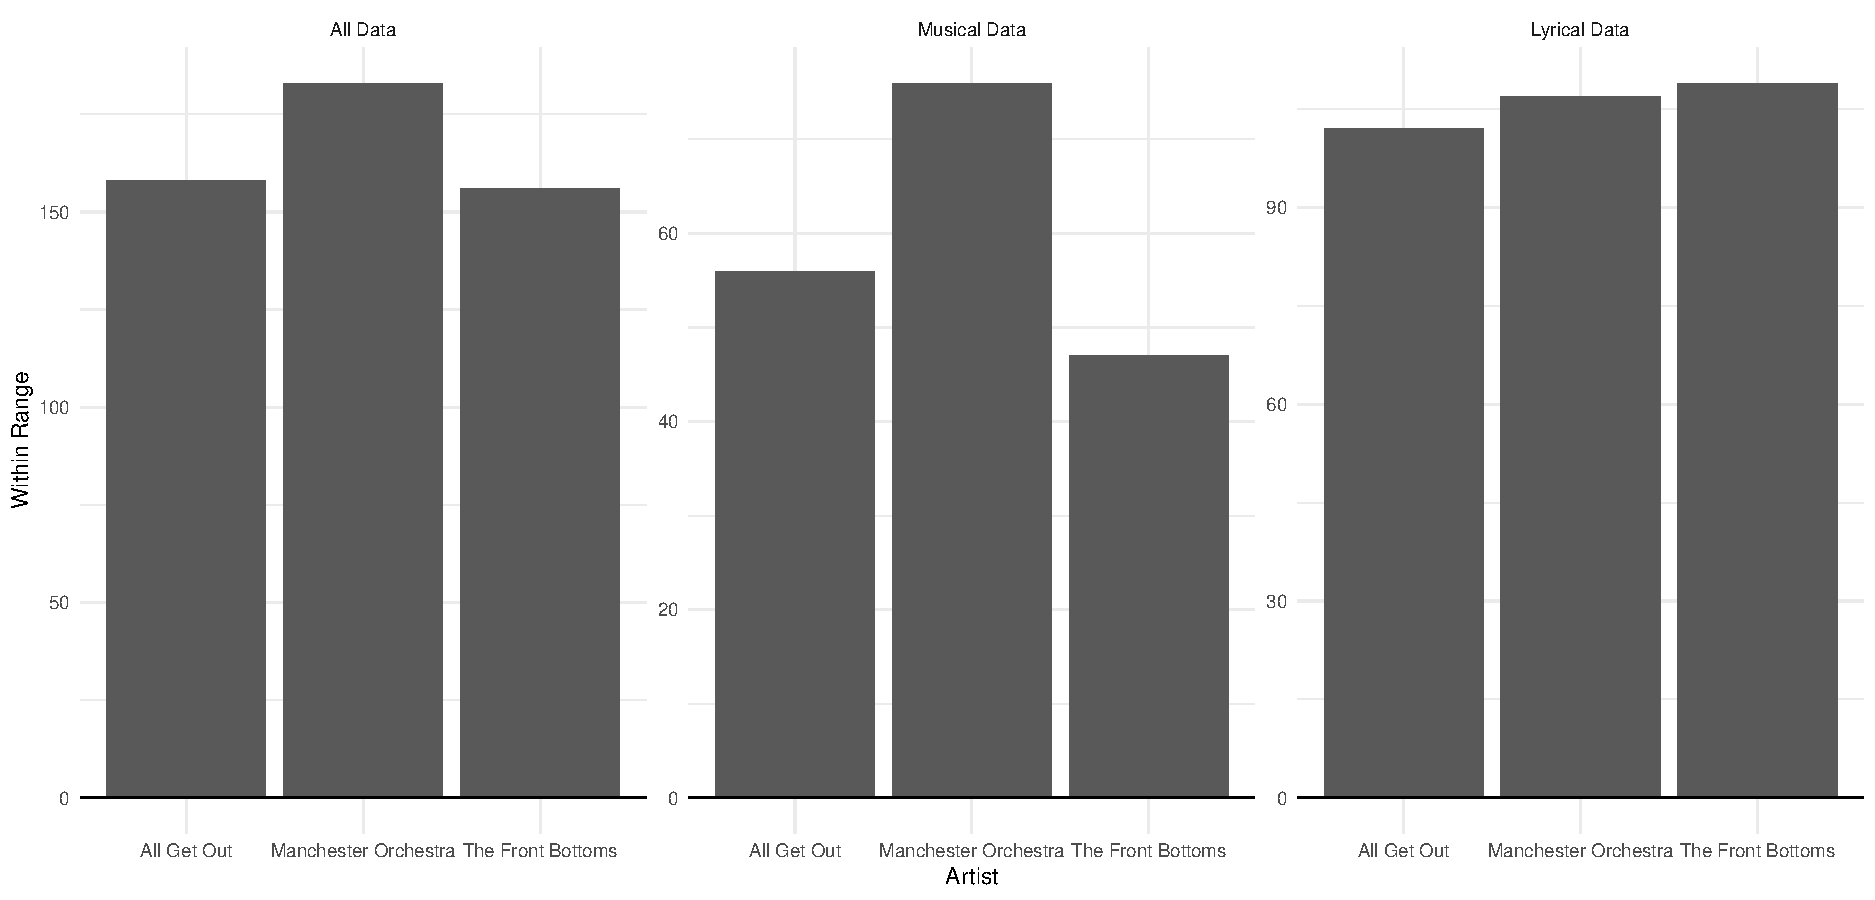
\includegraphics[width=\maxwidth]{figure/unnamed-chunk-3-1} 
\end{knitrout}
\caption*{Comparison of All Data, Musical Data, and Lyrical Data}
\label{Graph}
\end{center}
\end{figure}

\begin{table}[H]
\begin{center}
\caption*{\textbf{All Data}}
\begin{tabular}{rlrrr}
  \hline
 & Artist & Within Range & Outlying & Out of Range \\ 
  \hline
  1 & All Get Out & 158 & 17 & 22 \\ 
  2 & Manchester Orchestra & 183 & 11 & 3 \\ 
  3 & The Front Bottoms & 156 & 11 & 30 \\ 
   \hline
\end{tabular}
\caption*{Range of all Features Similar to \emph{Allentown} by Artist}
\end{center}
\label{AllTable}
\end{table}

\begin{table}[H]
\centering
\caption*{\textbf{Musical Data}}
\begin{tabular}{rlrrr}
  \hline
 & Artist & Within Range & Outlying & Out of Range \\ 
  \hline
1 & All Get Out & 56 & 10 & 12 \\ 
  2 & Manchester Orchestra & 76 & 2 & 0 \\ 
  3 & The Front Bottoms & 47 & 5 & 26 \\ 
   \hline
\end{tabular}
\caption*{Range of Musical Features Similar to \emph{Allentown} by Artist}
\label{MusicalTable}
\end{table}

\begin{table}[H]
\centering
\caption*{\textbf{Lyrical Data}}
\begin{tabular}{rlrrr}
  \hline
 & Artist & Within Range & Outlying & Out of Range \\ 
  \hline
1 & All Get Out & 102 & 7 & 10 \\ 
  2 & Manchester Orchestra & 107 & 9 & 3 \\ 
  3 & The Front Bottoms & 109 & 6 & 4 \\ 
   \hline
\end{tabular}
\caption*{Range of Lyrical Features Similar to \emph{Allentown} by Artist}
\label{LyricalTable}
\end{table}

\twocolumn

\section{Discussion}

%%%%%%%%%%%%%%%%%%%%%%%%%%%%%%%%%%%%%%%%%%%%%%%%%%%%%%%%%%%%%%%%%%%%%%%%%%%%%%%%
% Bibliography
%%%%%%%%%%%%%%%%%%%%%%%%%%%%%%%%%%%%%%%%%%%%%%%%%%%%%%%%%%%%%%%%%%%%%%%%%%%%%%%%

\vspace{2em}
\begin{tiny}
\bibliography{bib}
\end{tiny}
\end{multicols}

\end{document}
